\documentclass[11pt]{article}

\usepackage[margin=1in]{geometry}
\usepackage{graphicx}
\usepackage{booktabs}
\usepackage{url}
\usepackage{hyperref}
\usepackage{xcolor}
\usepackage{amsmath}

\title{Tiny-GEMM: Packed INT4 Triton GEMM for Decode-Heavy LLM Inference}
\author{Robert Zhang}
\date{}

\begin{document}
\maketitle

\begin{abstract}
Small-batch LLM decoding is dominated by narrow GEMMs that stress memory
bandwidth and launch overhead rather than peak FLOPs. We present Tiny-GEMM, a
packed INT4 GEMM kernel in Triton targeted at decode-heavy shapes, and a
measurement-driven analysis of when quantization helps or hurts. We compare
FP16, dequantized FP16, and INT4 fused kernels, attribute performance using
hardware counters, and isolate dequantization overhead with microbenchmarks.
Results on an A10G show substantial gains for wide FFN decode shapes while
highlighting regimes where dequant overhead dominates. We provide a reproducible
evaluation harness and a focused set of figures that connect kernel behavior to
systems-level inference constraints.
\end{abstract}

\section{Introduction}
LLM inference workloads differ sharply from training: decoding operates at batch
sizes of 1--8 with skinny matrices and tight latency budgets. These shapes are
often memory-bound, and naive quantization can underperform if dequantization
overhead is not amortized. This work explores packed INT4 GEMM in Triton and
provides a systems-oriented evaluation emphasizing utilization, bottleneck
regimes, and deployment-relevant shapes.

\paragraph{Contributions.}
\begin{itemize}
  \item A packed INT4 GEMM kernel optimized for decode-heavy shapes with static
        configuration selection.
  \item A multi-baseline evaluation (FP16, dequantized FP16, INT4 fused) that
        separates quantization benefits from kernel effects.
  \item Hardware-counter evidence and microbenchmarks that explain when INT4
        helps or hurts.
\end{itemize}

\section{Background and Motivation}
Decode GEMMs (e.g., Q/K/V projections and FFN layers) typically use $M \in
\{1,2,4,8\}$ and hidden dimensions in the 4K--16K range. For these shapes, the
dominant costs are memory movement and kernel launch overhead, not peak compute.
This motivates INT4 weight packing and fused computation to reduce traffic and
improve utilization.

\section{Method}
We implement packed INT4 GEMM in Triton with per-tensor quantization and
bit-packed weight tensors. The kernel unpacks INT4 values into FP32 accumulators
inside the kernel and uses static configurations keyed by shape family and batch
bucket. We evaluate three baselines:

\begin{itemize}
  \item \textbf{FP16}: \texttt{torch.matmul} as the standard deployment baseline.
  \item \textbf{Dequantized FP16}: INT4 quantize $\rightarrow$ dequant $\rightarrow$ FP16 GEMM.
  \item \textbf{INT4 fused}: packed INT4 GEMM kernel (Tiny-GEMM).
\end{itemize}

\section{Experimental Setup}
All experiments run on an NVIDIA A10G GPU. We focus on decode shapes derived
from Llama-style models: Q/FFN projections with $K,N$ in $\{4096, 14336\}$ and
KV projections with $N=1024$. Profiling uses Nsight Compute; wall-clock timings
are reported from the benchmark harness (profilers replay kernels and inflate
timings).

\section{Results}

\subsection{Where Does INT4 Help?}
We first identify the regime where INT4 improves decode performance.
Figure~\ref{fig:speedup-vs-n} shows speedup vs FP16 as $N$ increases (fixed
$K=4096$). INT4 underperforms on narrow projections but provides strong gains
for wide FFN layers. Figure~\ref{fig:family-latency} groups results by layer
family, showing the same trend across M=1 and M=8.

\begin{figure}[t]
  \centering
  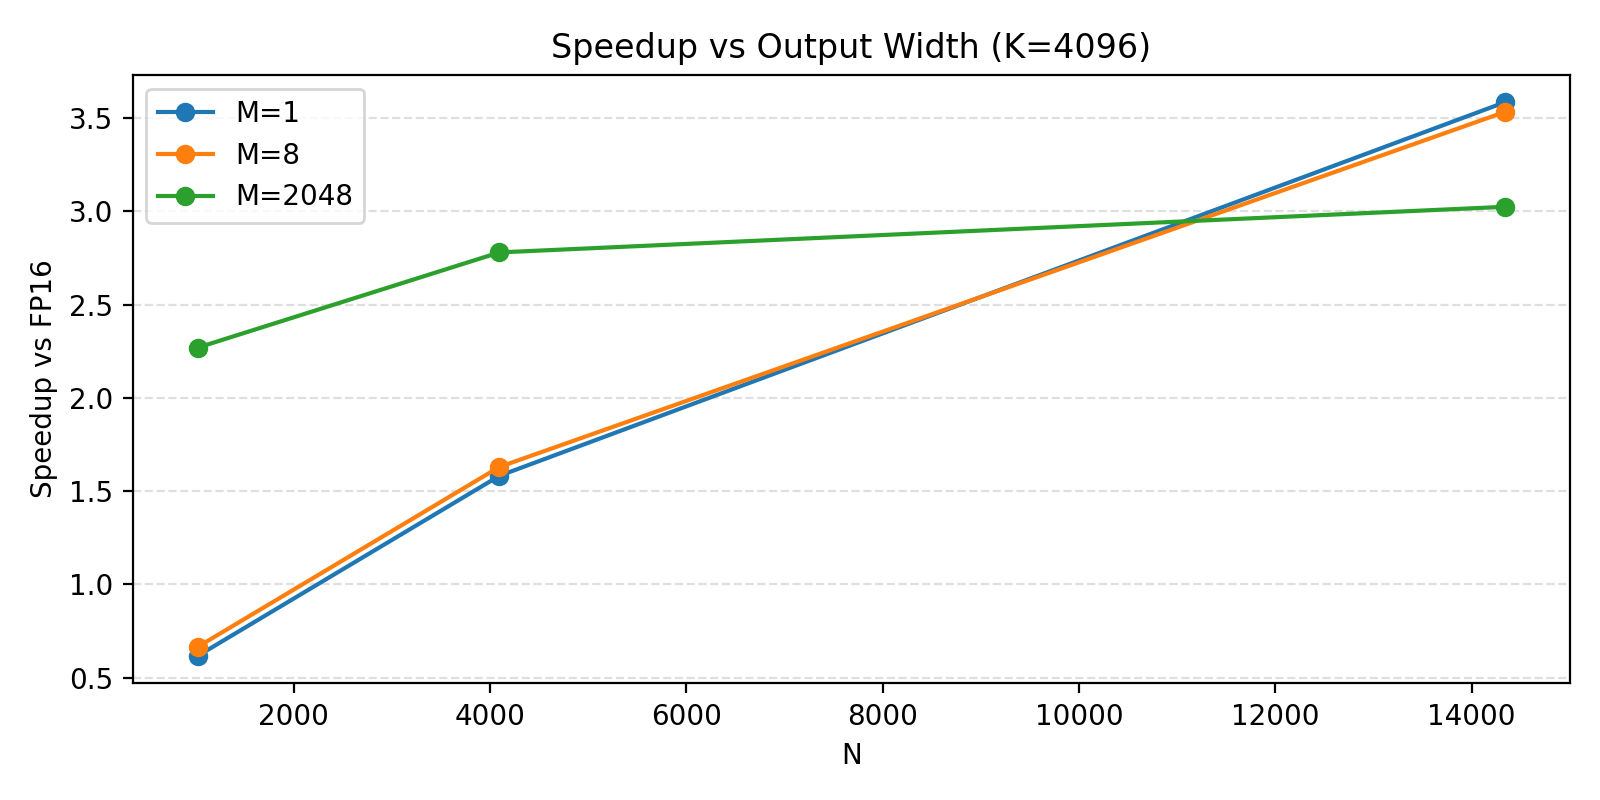
\includegraphics[width=0.75\linewidth]{../figures/speedup_vs_n_k4096.png}
  \caption{Speedup vs output width $N$ (decode shapes, $K=4096$).}
  \label{fig:speedup-vs-n}
\end{figure}

\begin{figure}[t]
  \centering
  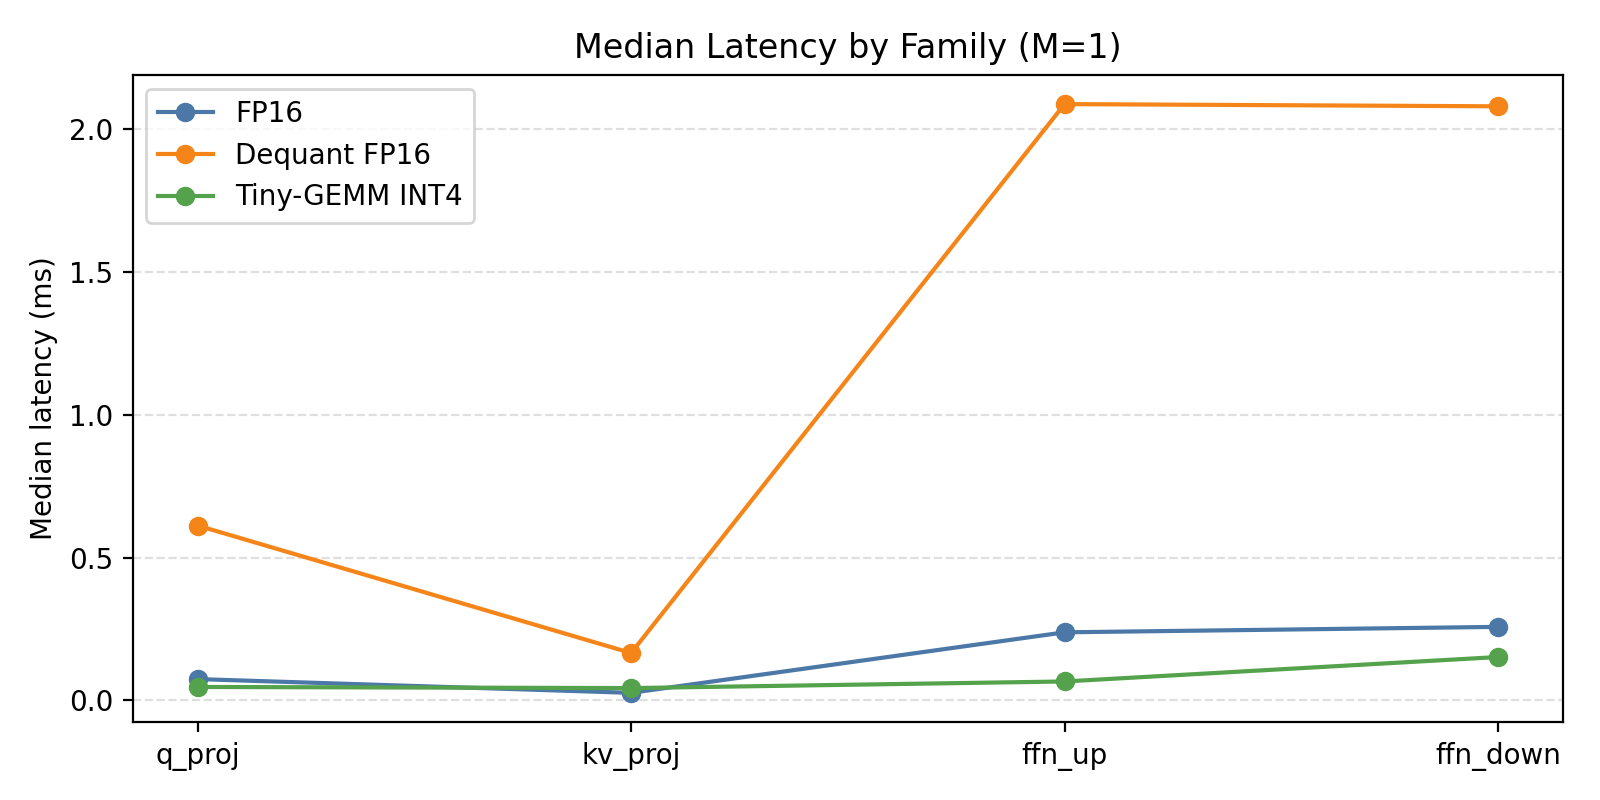
\includegraphics[width=0.8\linewidth]{../figures/family_latency_m1.png}
  \caption{Latency by shape family (M=1).}
  \label{fig:family-latency}
\end{figure}

\subsection{Why Does INT4 Help (or Hurt)?}
We isolate dequantization overhead and attribute bottleneck shifts. The
dequantization microbenchmark (Figure~\ref{fig:dequant-breakdown}) shows that
fixed INT4 overhead dominates narrow projections, explaining regressions on
KV-like shapes. Hardware counters provide a complementary view: INT4 shifts
utilization compared to FP16 (Figure~\ref{fig:util-compare}), while a roofline
scatter illustrates the memory-bound regime (Figure~\ref{fig:roofline}).

\begin{figure}[t]
  \centering
  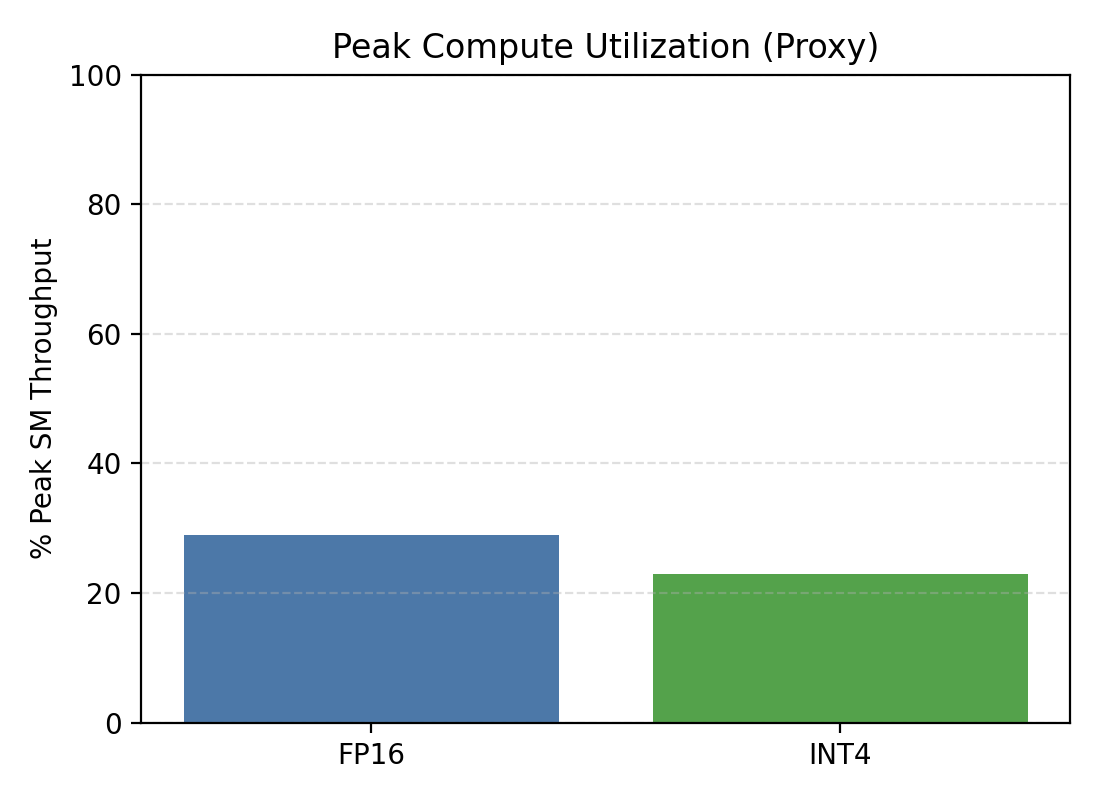
\includegraphics[width=0.55\linewidth]{../figures/peak_compute_utilization.png}
  \caption{Peak compute utilization proxy (SM throughput) for FP16 vs INT4.}
  \label{fig:peak-compute}
\end{figure}

\begin{figure}[t]
  \centering
  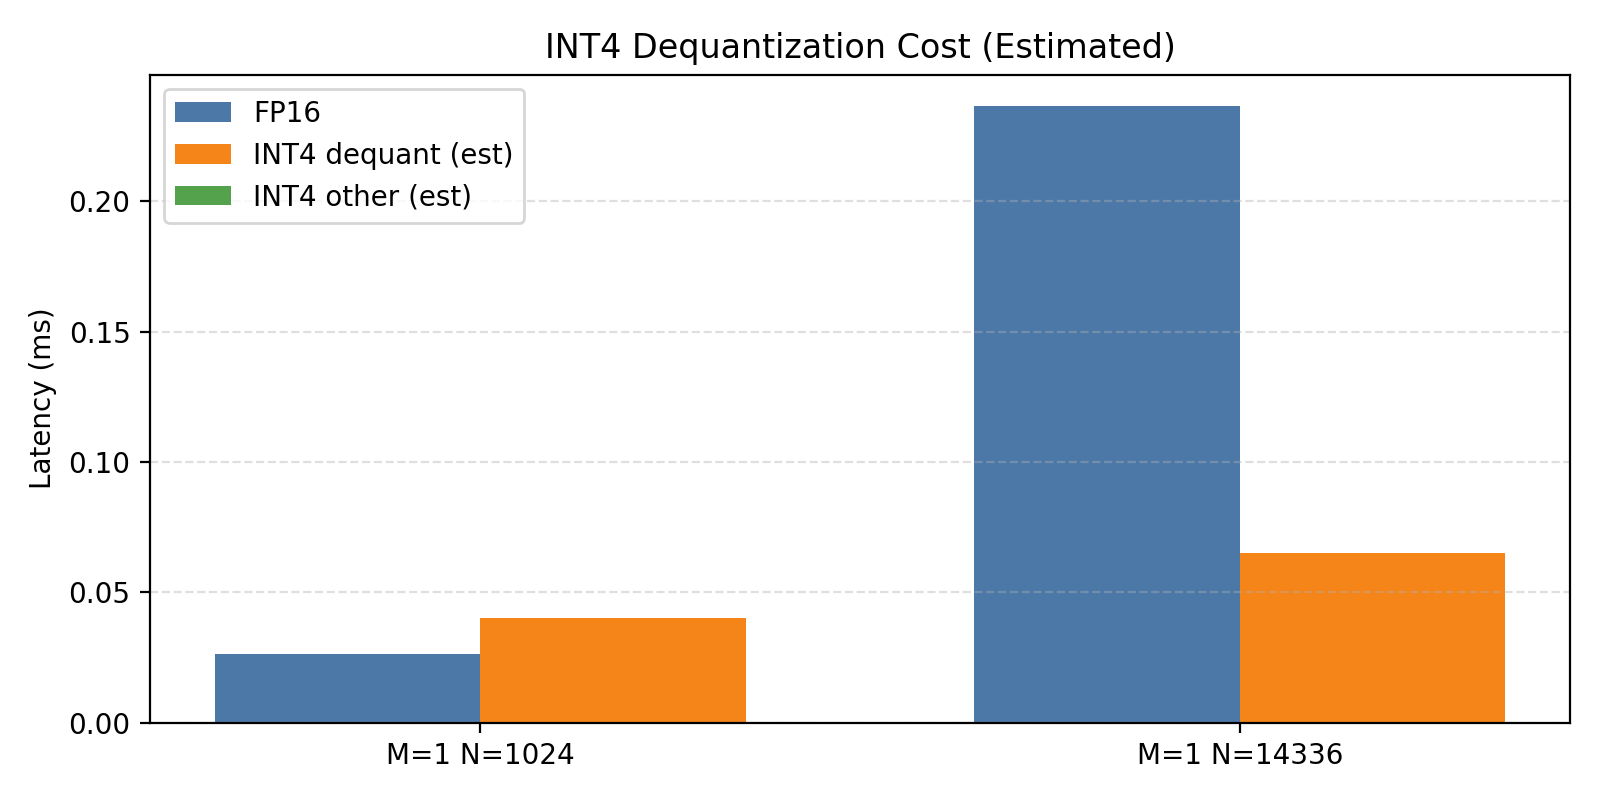
\includegraphics[width=0.75\linewidth]{../figures/dequant_breakdown.png}
  \caption{Dequantization breakdown for representative decode shapes.}
  \label{fig:dequant-breakdown}
\end{figure}

\begin{figure}[t]
  \centering
  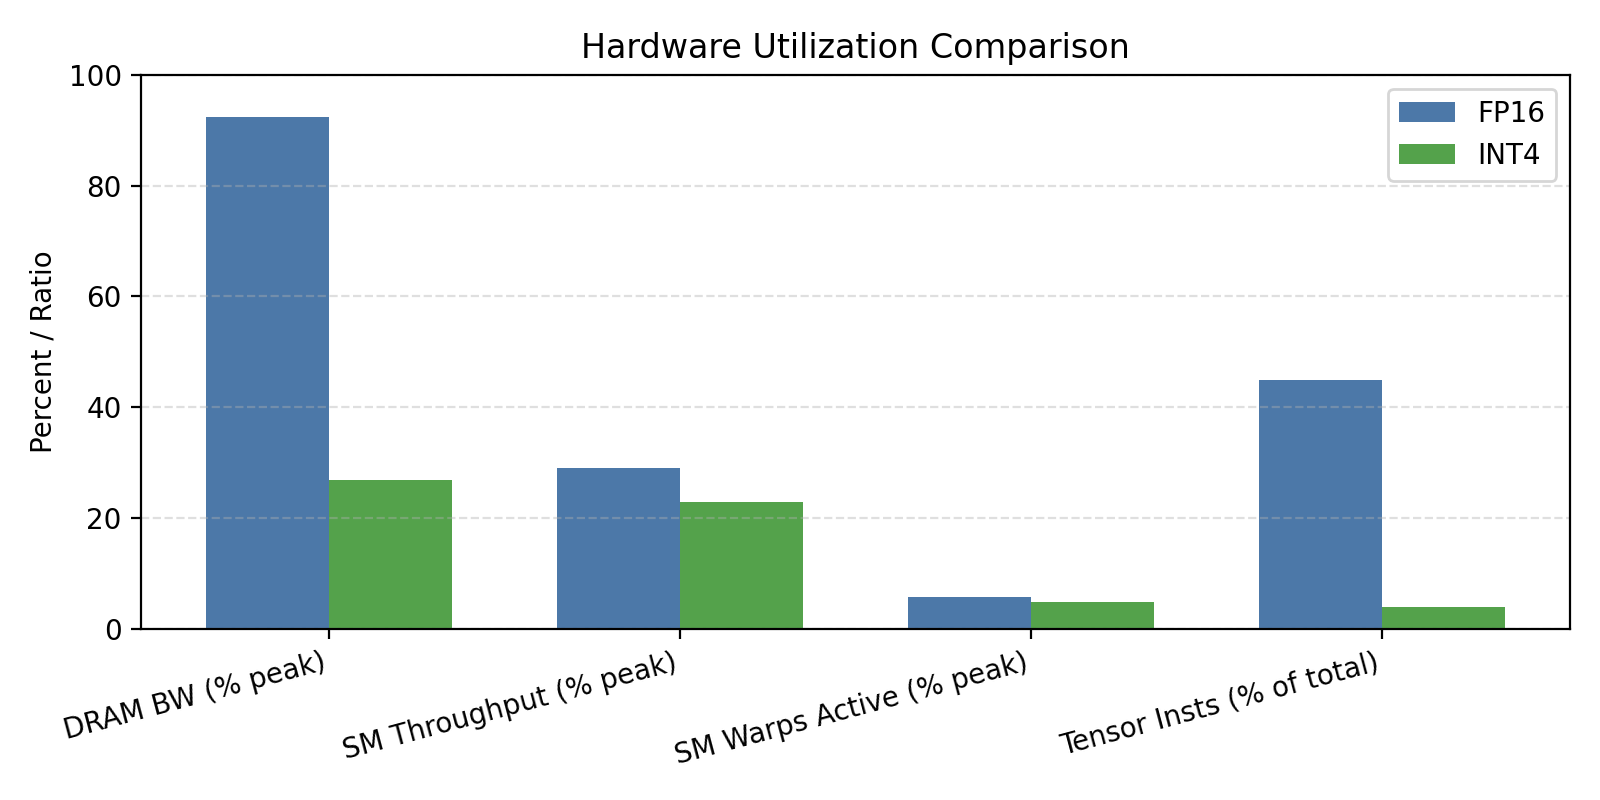
\includegraphics[width=0.75\linewidth]{../figures/ncu_utilization_comparison.png}
  \caption{Hardware utilization comparison (FP16 vs INT4).}
  \label{fig:util-compare}
\end{figure}

\begin{figure}[t]
  \centering
  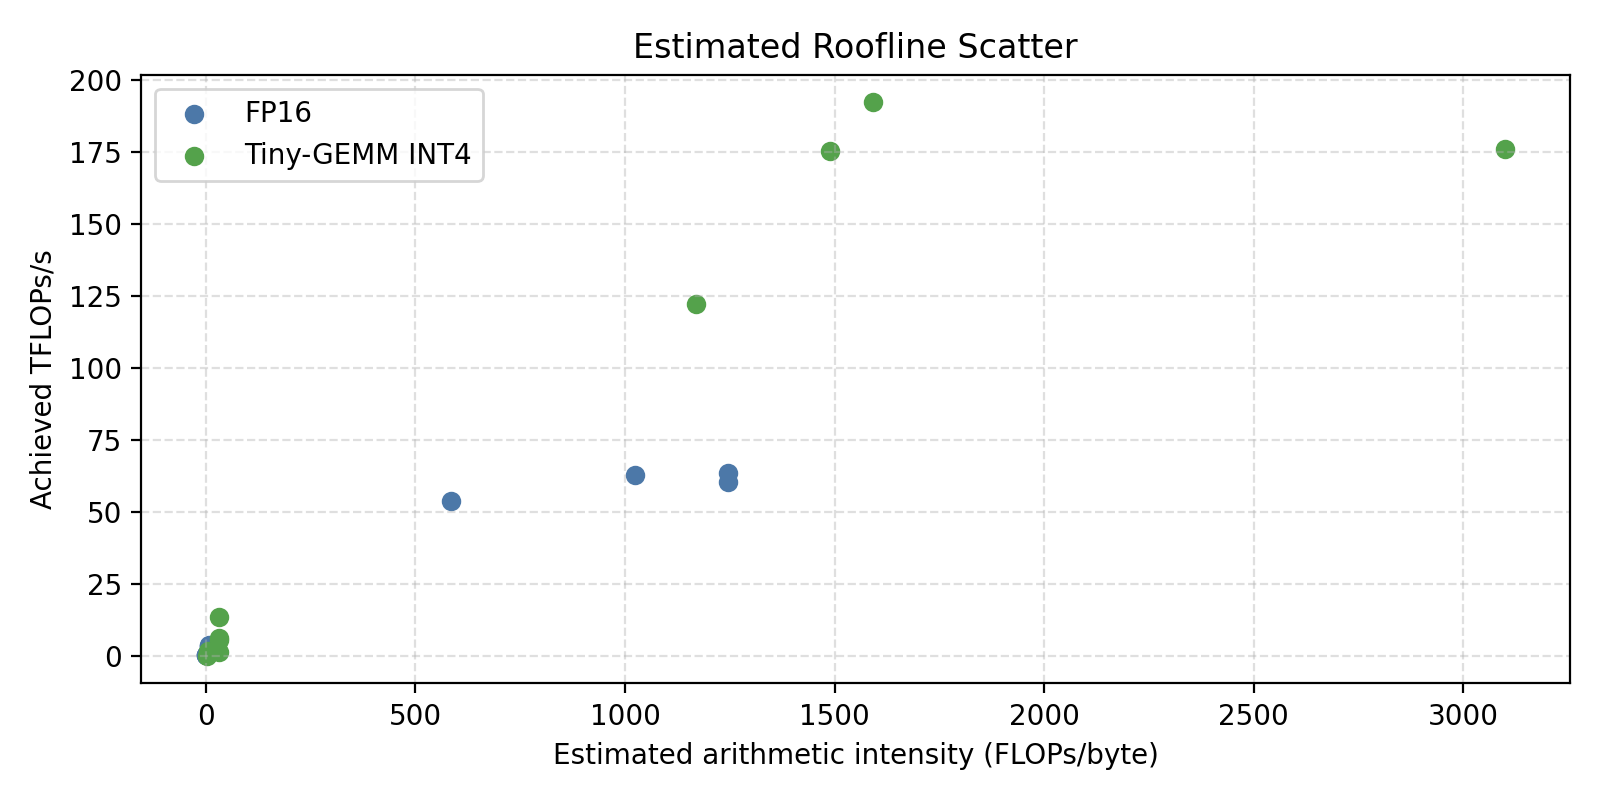
\includegraphics[width=0.7\linewidth]{../figures/roofline_scatter.png}
  \caption{Estimated roofline scatter (arithmetic intensity vs TFLOPs).}
  \label{fig:roofline}
\end{figure}

\subsection{When Does INT4 Help in Systems Terms?}
We examine batch scaling and throughput to connect kernel behavior to decode
latency constraints. Figure~\ref{fig:batch-scaling} shows latency vs batch size
for a representative decode shape; Figure~\ref{fig:tps} reports tokens/sec.

\begin{figure}[t]
  \centering
  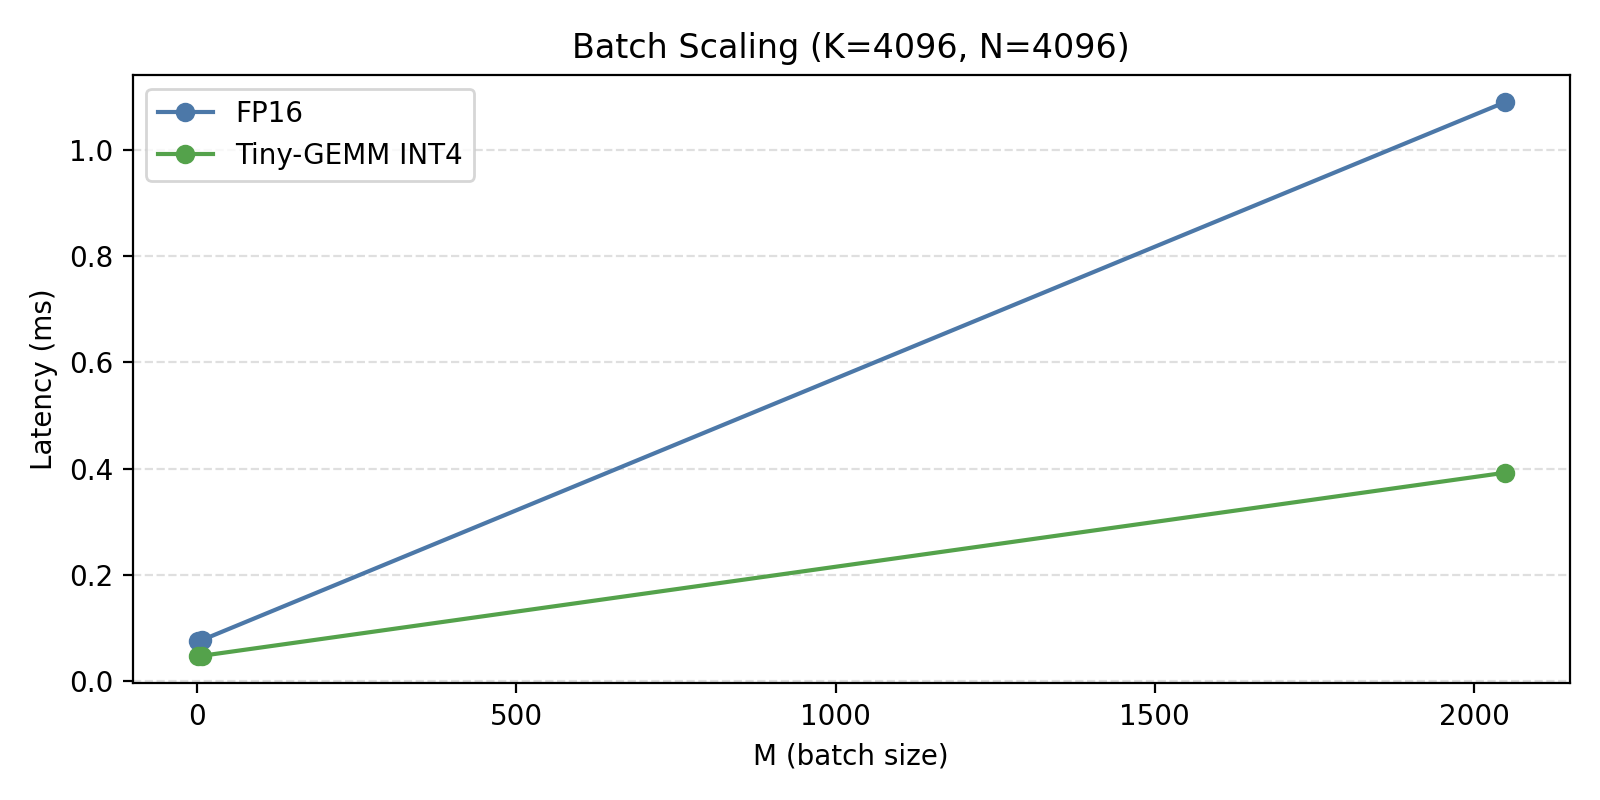
\includegraphics[width=0.75\linewidth]{../figures/batch_scaling_k4096_n4096.png}
  \caption{Batch scaling for decode ($K=N=4096$).}
  \label{fig:batch-scaling}
\end{figure}

\begin{figure}[t]
  \centering
  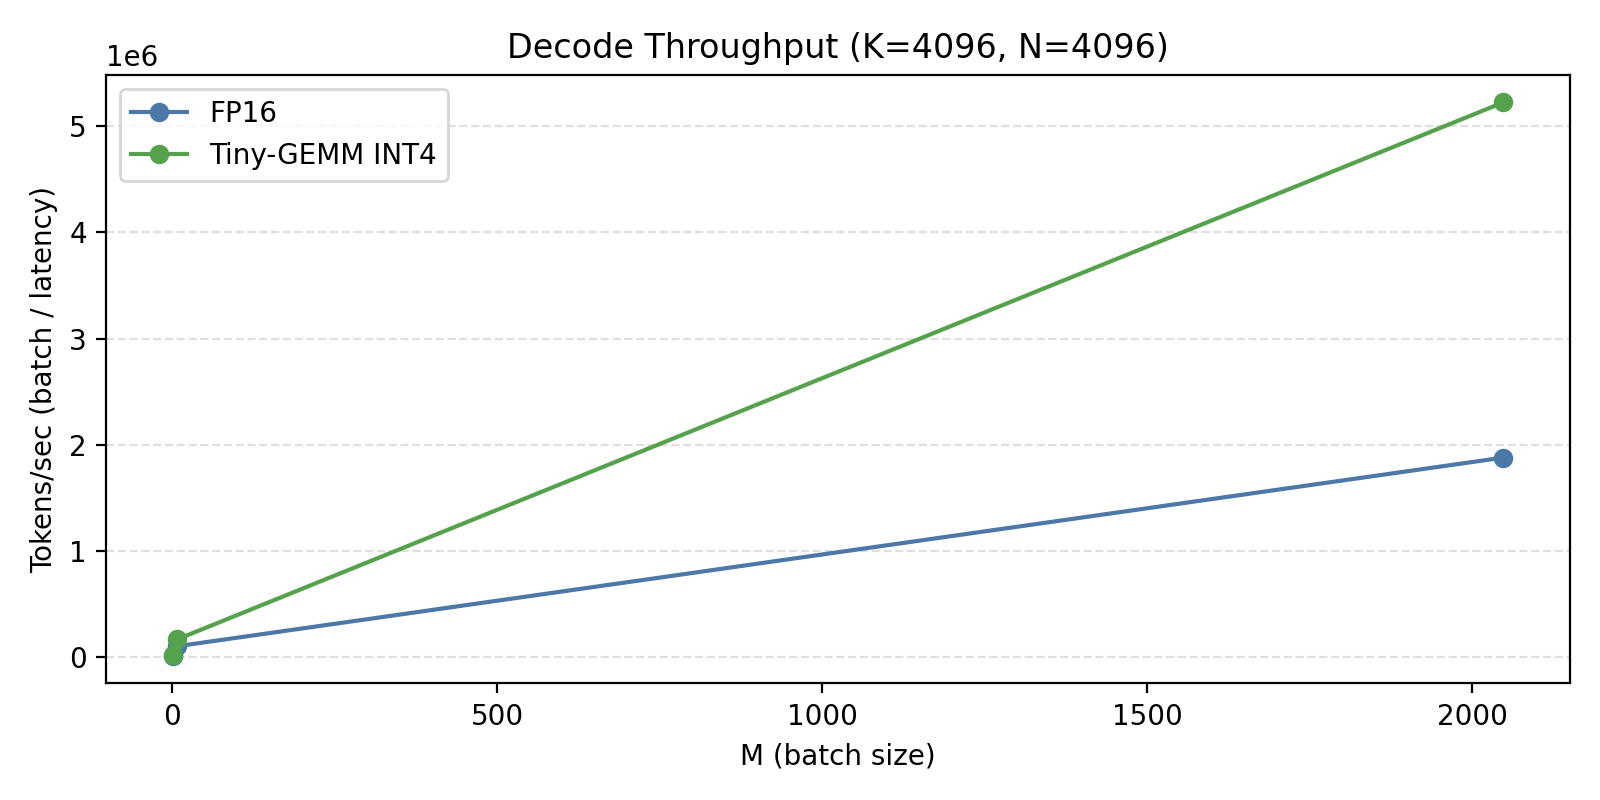
\includegraphics[width=0.75\linewidth]{../figures/tokens_per_sec_k4096_n4096.png}
  \caption{Decode throughput (tokens/sec) vs batch size.}
  \label{fig:tps}
\end{figure}

\subsection{Prefill vs Decode}
We compare prefill-like ($M \gg 1$) and decode-like ($M \le 8$) regimes using a
fixed shape family grouping. INT4 benefits are stronger in decode for wide FFN
layers but remain mixed for narrow projections.

\begin{figure}[t]
  \centering
  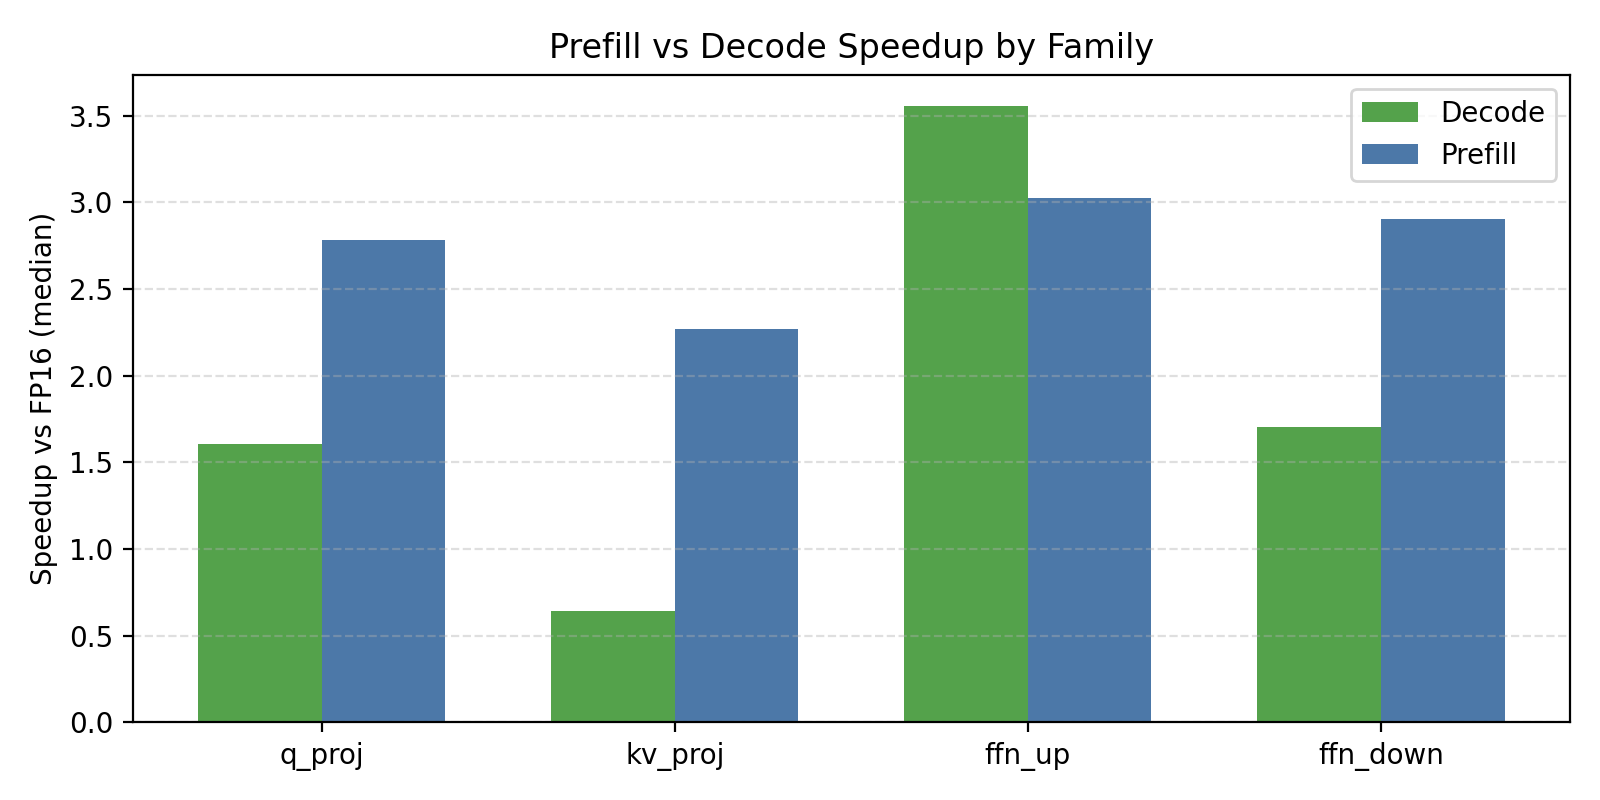
\includegraphics[width=0.75\linewidth]{../figures/prefill_vs_decode_speedup.png}
  \caption{Prefill vs decode speedup by family.}
  \label{fig:prefill-decode}
\end{figure}

\subsection{Regime Map and Kernel Composition}
To summarize regimes, we include a decode heatmap (Figure~\ref{fig:heatmap}) and
kernel time composition (Figure~\ref{fig:kernel-time}).

\begin{figure}[t]
  \centering
  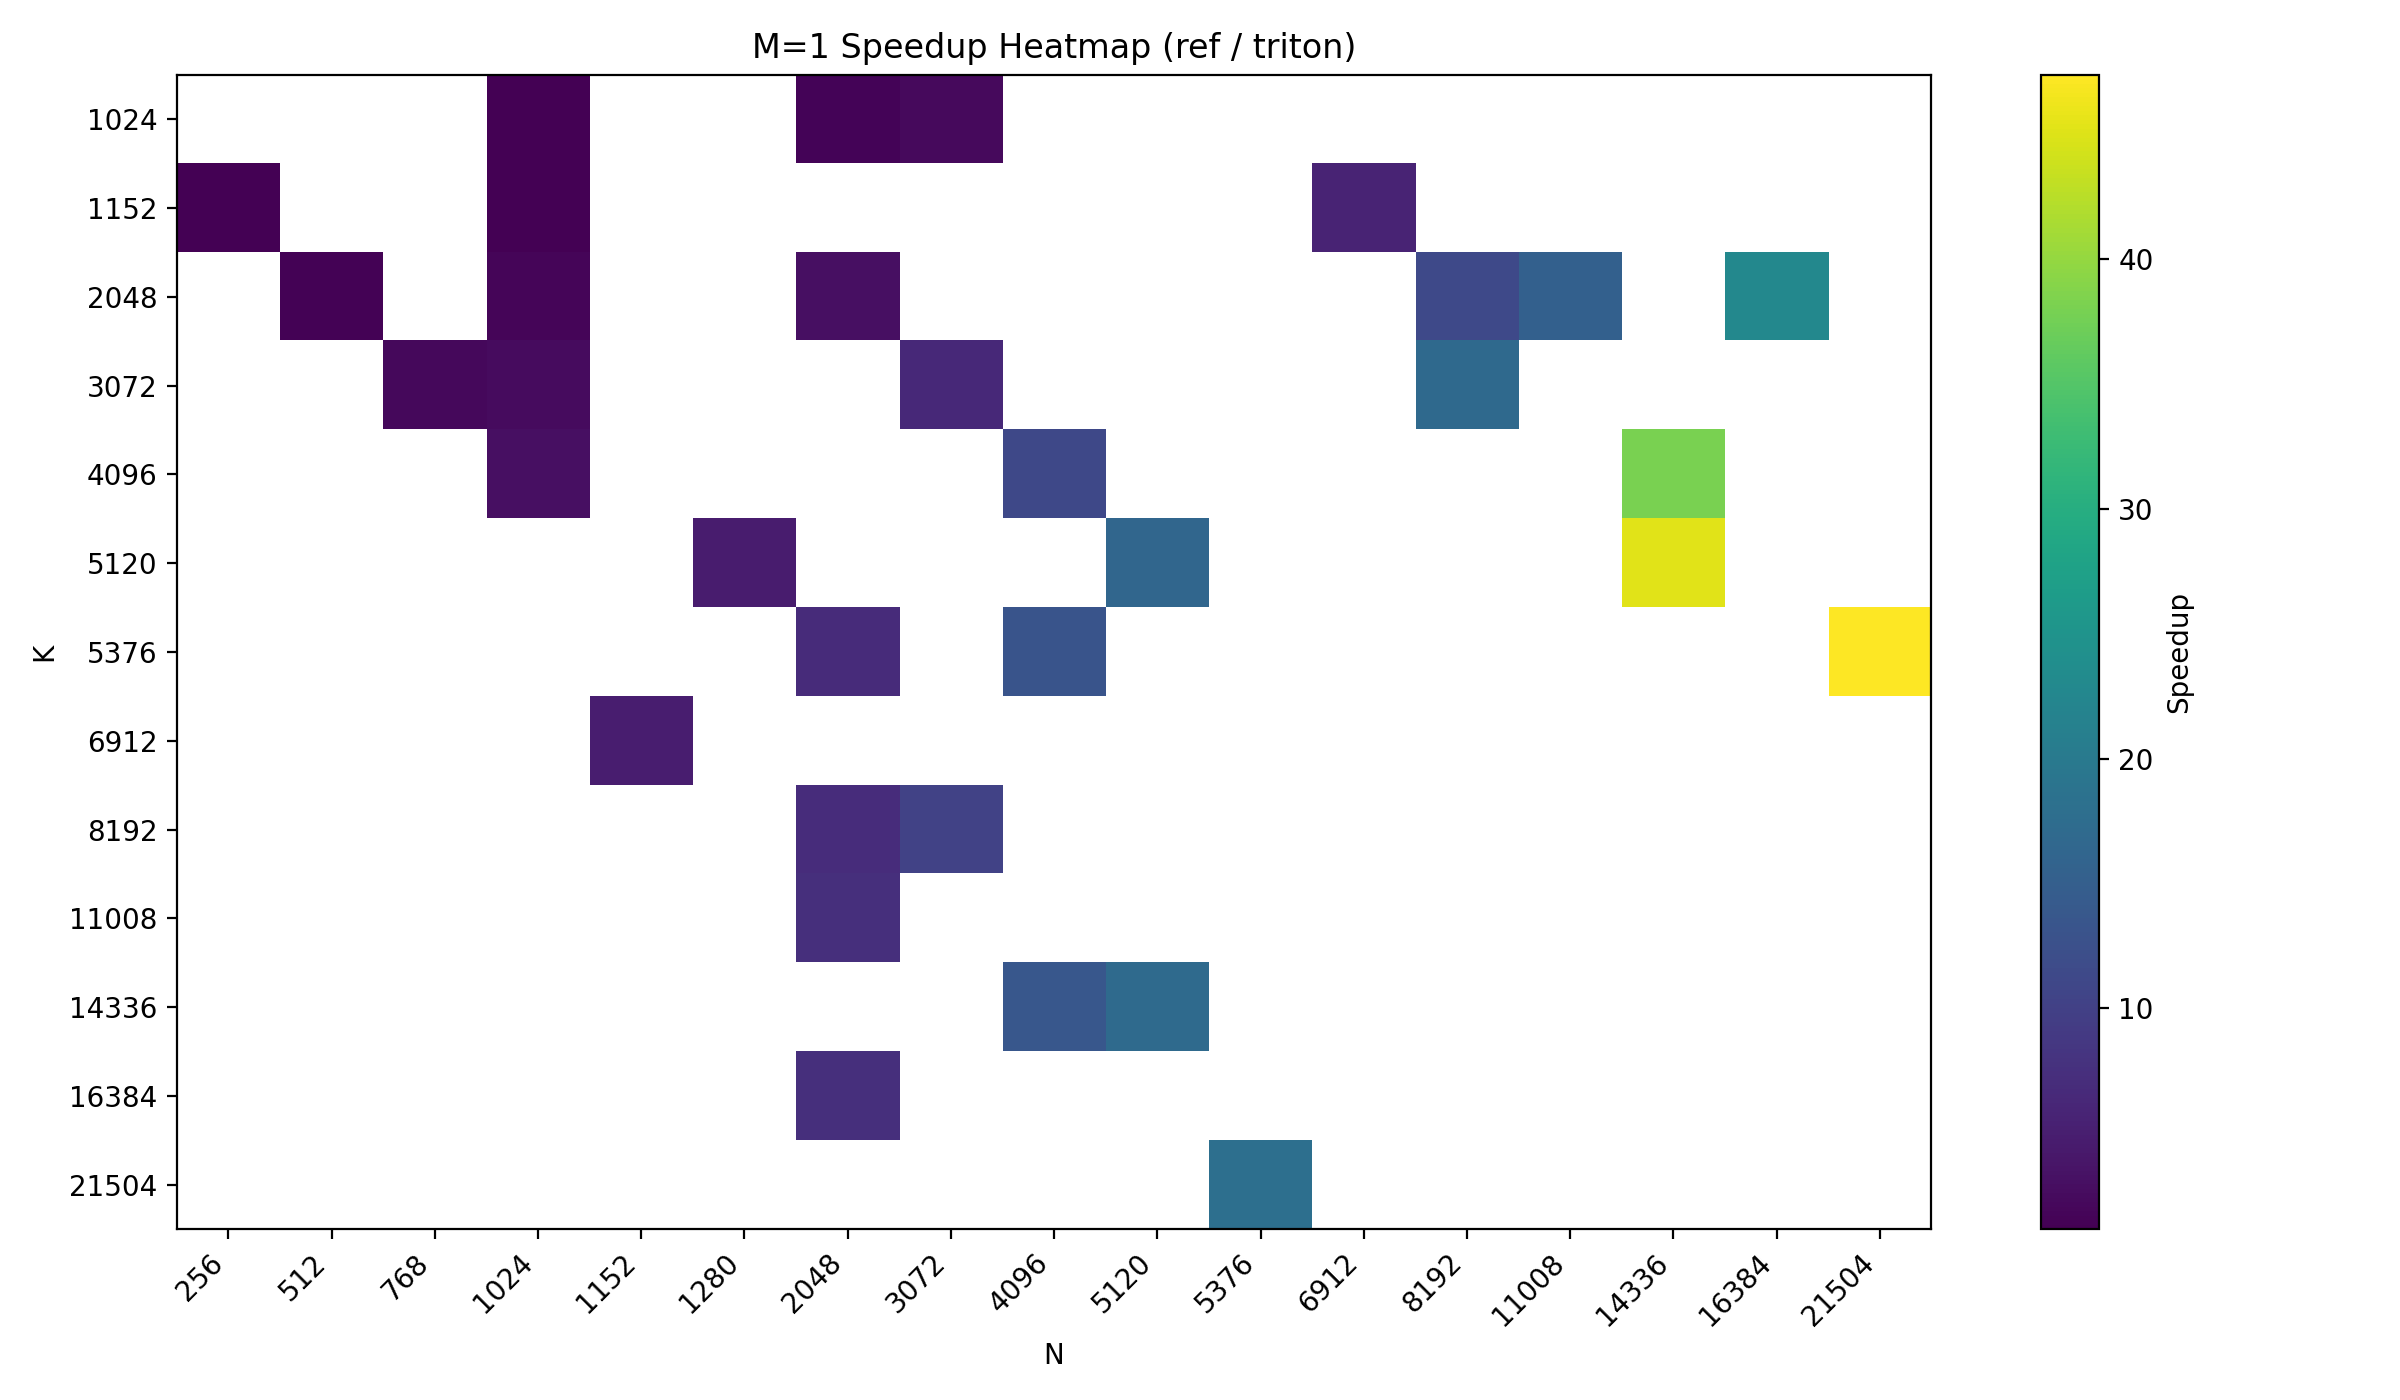
\includegraphics[width=0.75\linewidth]{../figures/int4_speedup_heatmap_m1.png}
  \caption{Decode regime map (M=1) across $K$ and $N$.}
  \label{fig:heatmap}
\end{figure}

\begin{figure}[t]
  \centering
  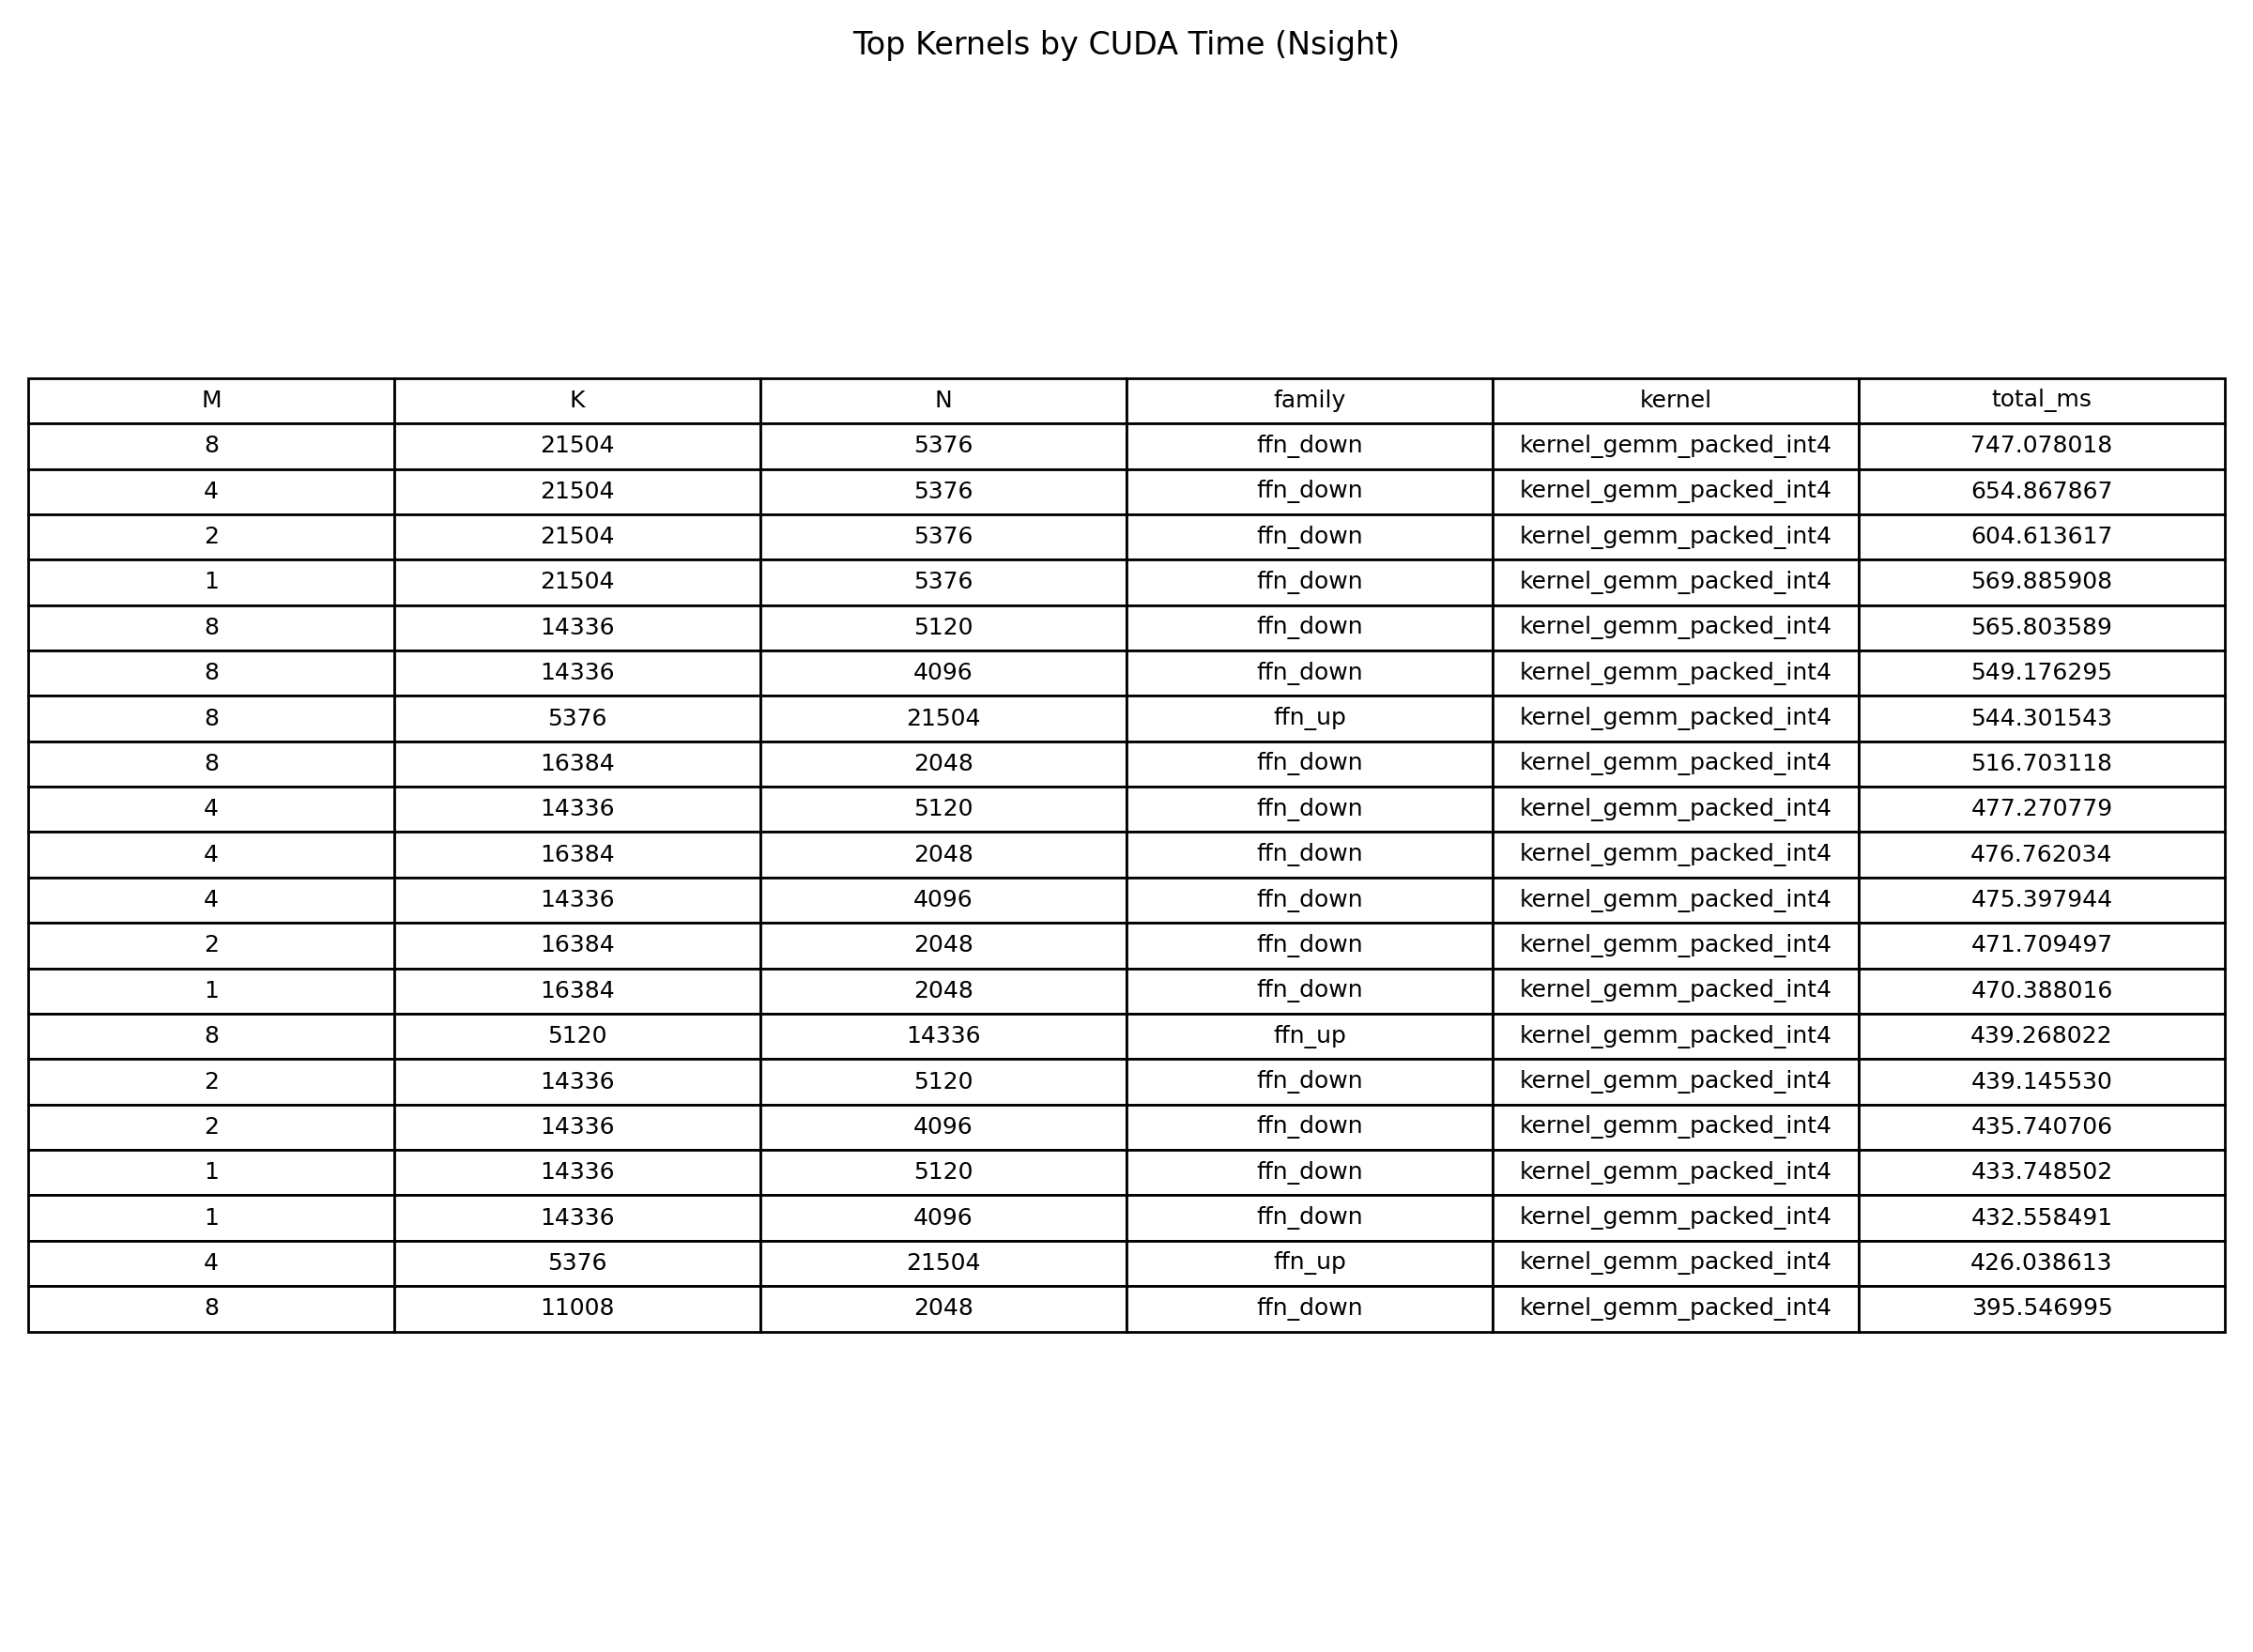
\includegraphics[width=0.75\linewidth]{../figures/top_kernels_by_cuda_time.png}
  \caption{Kernel time composition for top shapes (Nsight Systems).}
  \label{fig:kernel-time}
\end{figure}

\section{Discussion}
The results support a clear regime interpretation: INT4 helps when arithmetic
intensity is sufficient to amortize dequantization and when memory traffic is a
dominant bottleneck. For narrow projections (e.g., KV), fixed overheads and
limited parallelism can outweigh the bandwidth savings. These findings align
with practical inference constraints in decode-heavy serving.

\section{Limitations}
This study targets a single GPU and a fixed set of decode shapes. The kernel is
not yet optimized for all regimes (e.g., split-K for $M=1$), and the INT4 kernel
does not currently exploit tensor core INT4 MMA pipelines. Future work should
extend to additional hardware (L4/A100), incorporate split-K or persistent
kernel strategies, and explore INT8/FP8 comparisons.

\section{Conclusion}
Tiny-GEMM demonstrates that packed INT4 kernels can significantly improve
decode performance for wide FFN shapes while exposing the boundaries where
dequant overhead dominates. By pairing multi-baseline benchmarks with hardware
counters and targeted microbenchmarks, we provide a systems-level narrative of
when and why INT4 helps in real inference settings.

\end{document}
